% !TEX TS-program = pdflatex
% !TEX encoding = UTF-8 Unicode

\documentclass[a4paper, titlepage=false, parskip=full-, 10pt]{scrartcl}

\usepackage[utf8]{inputenc}
\usepackage[T1]{fontenc}
\usepackage[english, ngerman]{babel}
\usepackage{babelbib}
\usepackage{hyperref}
\usepackage{listings}
\usepackage{framed}
\usepackage{color}
\usepackage{graphicx}
\usepackage[normalem]{ulem}
\usepackage{cancel}
\usepackage{amsmath}
\usepackage{amssymb}
\usepackage{amsthm}
\usepackage{algorithm}
\usepackage{algorithmic}
\usepackage{geometry}
\usepackage{subfigure}
\geometry{a4paper, top=20mm, left=35mm, right=25mm, bottom=40mm}

\newcounter{tasknbr}
\setcounter{tasknbr}{1}
\newenvironment{task}[1]{{\bf Aufgabe \arabic {tasknbr}\stepcounter{tasknbr}} (#1):\begin{enumerate}}{\end{enumerate}}
\newcommand{\subtask}[1]{\item[#1)]}

% Listings -----------------------------------------------------------------------------
\definecolor{red}{rgb}{.8,.1,.2}
\definecolor{blue}{rgb}{.2,.3,.7}
\definecolor{lightyellow}{rgb}{1.,1.,.97}
\definecolor{gray}{rgb}{.7,.7,.7}
\definecolor{darkgreen}{rgb}{0,.5,.1}
\definecolor{darkyellow}{rgb}{1.,.7,.3}
\lstloadlanguages{C++,[Objective]C,Java}
\lstset{
escapeinside={§§}{§§},
basicstyle=\ttfamily\footnotesize\mdseries,
columns=fullflexible,
keywordstyle=\bfseries\color{blue},
commentstyle=\color{darkgreen},      
stringstyle=\color{red},
numbers=left,
numberstyle=\ttfamily\scriptsize\color{gray},
breaklines=true,
showstringspaces=false,
tabsize=4,
captionpos=b,
float=htb,
frame=tb,
frameshape={RYR}{y}{y}{RYR},
rulecolor=\color{black},
xleftmargin=15pt,
xrightmargin=4pt,
aboveskip=\bigskipamount,
belowskip=\bigskipamount,
backgroundcolor=\color{lightyellow},
extendedchars=true,
belowcaptionskip=15pt}

%% Enter current values here: %%
\newcommand{\lecture}{Computer Vision WS15/16}
\newcommand{\tutor}{}
\newcommand{\assignmentnbr}{2}
\newcommand{\students}{Julius Auer}
%%-------------------------------------%%

\begin{document}  
{\small \textsl{\lecture \hfill \tutor}}
\hrule
\begin{center}
\textbf{Übungsblatt \assignmentnbr}\\
[\bigskipamount]
{\small \students}
\end{center}
\hrule

\begin{task}{Kamerasensoren}
\subtask{1.1}
\emph{Nimm einen Fotoapparat (Handy, Webcam, ...) und nimm ein Foto von einer Szene mit (1) translatorischer und (2) rotatorischer Bewegung auf. Variiere dabei (i) die Lage des Bildsensors und (ii) die Belichtungsintensität. Zeige Beispielbilder für verschiedene Effekte die durch die Bewegung entstehen und benenne sie. Welchen Bildsensor hast Du vermutlich benutzt? Begründe (kurz)!}

Hmm, ohne Laborbedingungen herzustellen ist ''\emph{zeige Beispielbilder für verschiedene Effekte}'' ziemlich schwierig: allein ''aus dem Handgelenk'' mit ausreichender Geschwindigkeit zu rotieren, bringt mich schon an den Rand meiner motorischen Fähigkeiten. Mit einem FUmanoid-Kopf hätte man zwar schön eine Translation unter Laborbedingungen durchführen können, aber keine Rotation (nicht ausreichendd Freiheitsgrade). Außerdem bin ich für ein größeres Experiment gerade zu faul.

Davon abgesehen ist der einzige Effekt der mir einfällt und der in diesem Kontext ''\emph{durch die Bewegung}'' entstanden ist und der  hier nachgewiesen werden könnte der Rolling-Shutter-Effekt. Ich wüsste gar nicht, auf welche anderen Effekte die Frage abzielt? Quellen??

In Bezug auf ''\emph{Welchen Bildsensor hast Du vermutlich benutzt}'' könnte man - unabhängig von der Bewegung - noch auf Smear- und Blooming-Effekte achten.

Naja, nach einigen erfolglosen Versuchen Bildfehler auf Außenaufnahmen eines Zauns und meinem Parkett zu produzieren konnte ich immerhin einen Rolling-Shutter-Effekt (es handelt sich also wohl um einen älteren CMOS) beim Fotografieren eines mit einem Gewicht beschwerten 2-Adrigen Kupferkabels das an einer weißen Tür hängt erzeugen: Abbildung \ref{fig:1-1} zeigt den Versuchsaufbau, Abbildung \ref{fig:1-2} das Nicht-Auftreten des Effektes bei y-Translation und Abbildung \ref{fig:1-3} den Rolling-Shutter-Effekt bei x-Translation. Die Zeilenweise Verzerrung beim Rolling-Shutter-Effekt ist auch bei rotatorischer Bewegung (Abbildung \ref{fig:1-4}) zu erkennen. Nebeneinander sind jeweils Aufnahmen bei unterschiedlichen Lichtverhältnissen dargestellt - mein Unvermögen Smear- oder Blooming-Effekte zu produzieren könnte (muss aber nicht) zusätzlich auf einen CMOS hinweisen.

Lustig: mit zusätzliche Lichtquellen ist die Helligkeit deutlich reduziert und die Farbdarstellung deutlich verändert. Als Bildfehler würde ich das aber nicht bezeichnen.

\begin{figure}[!htpb]
\begin{center}
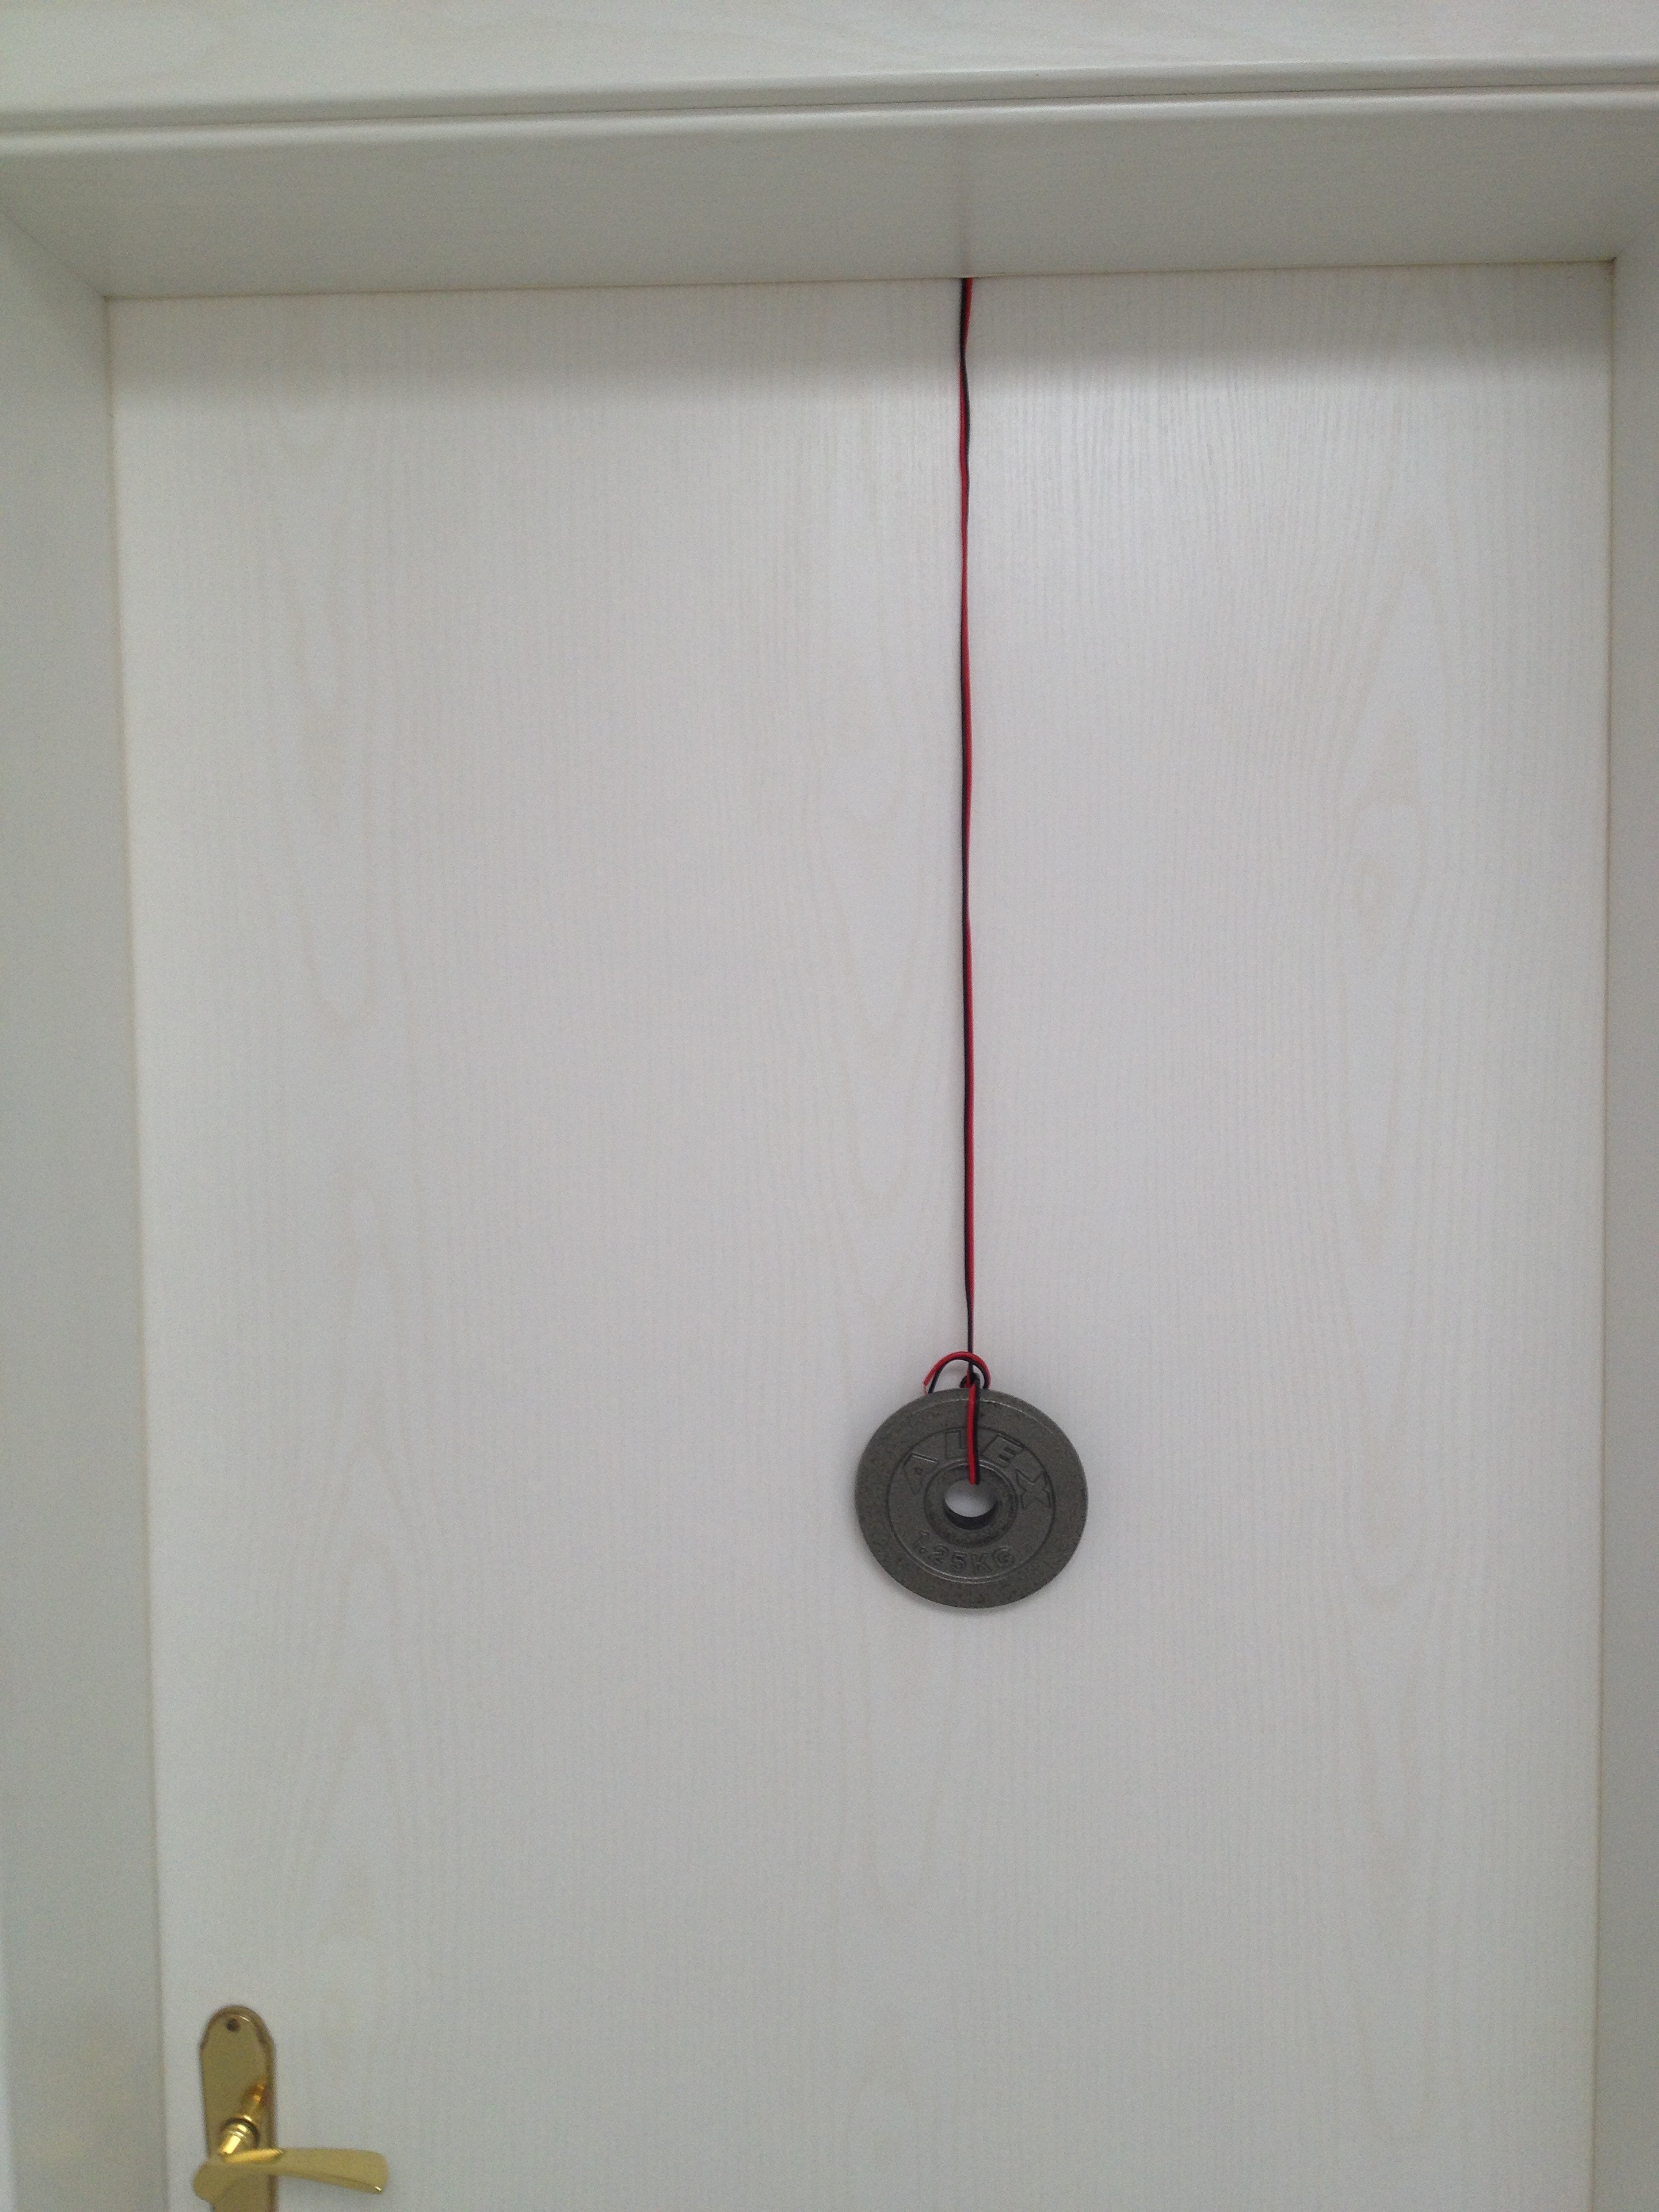
\includegraphics[width=7cm]{capture_1-1.jpg}
\end{center}
\caption{Ausgangssituation}
\label{fig:1-1}
\end{figure}

\begin{figure}[!htpb]
\begin{center}
\subfigure[Tageslicht]{
  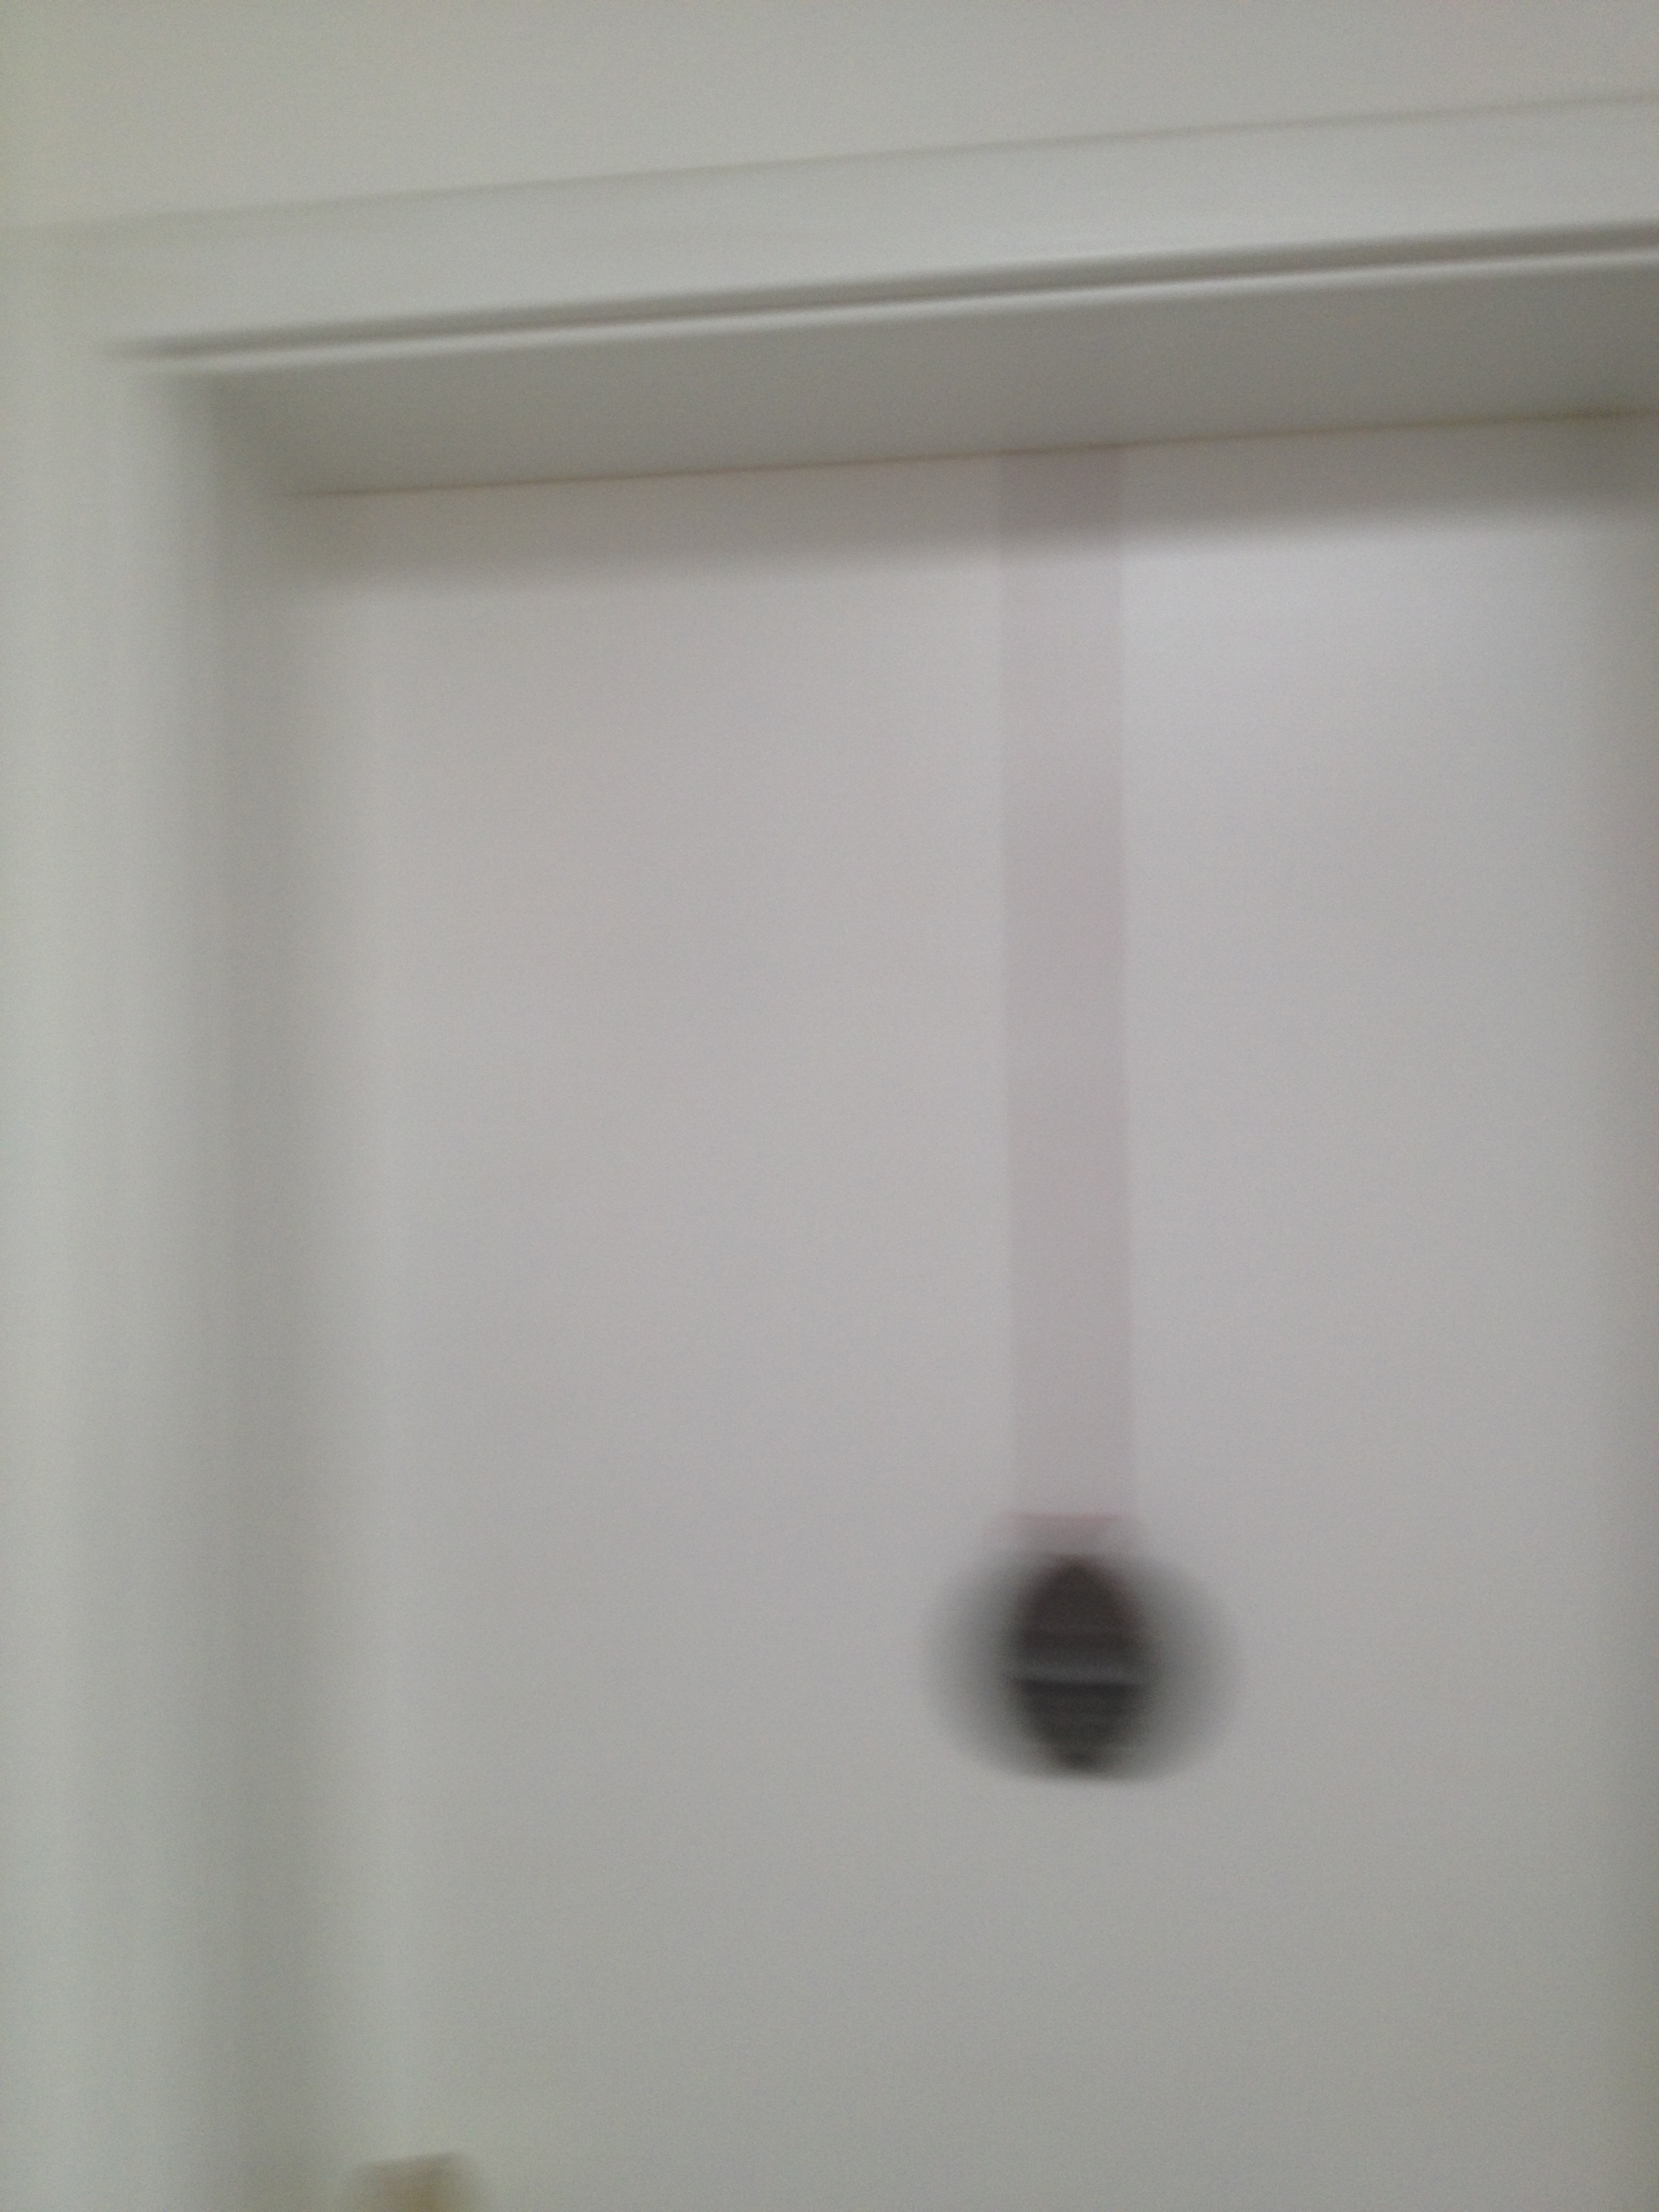
\includegraphics[width=7cm]{capture_1-2.jpg}
}
\subfigure[Blitz + Halogenspot]{
  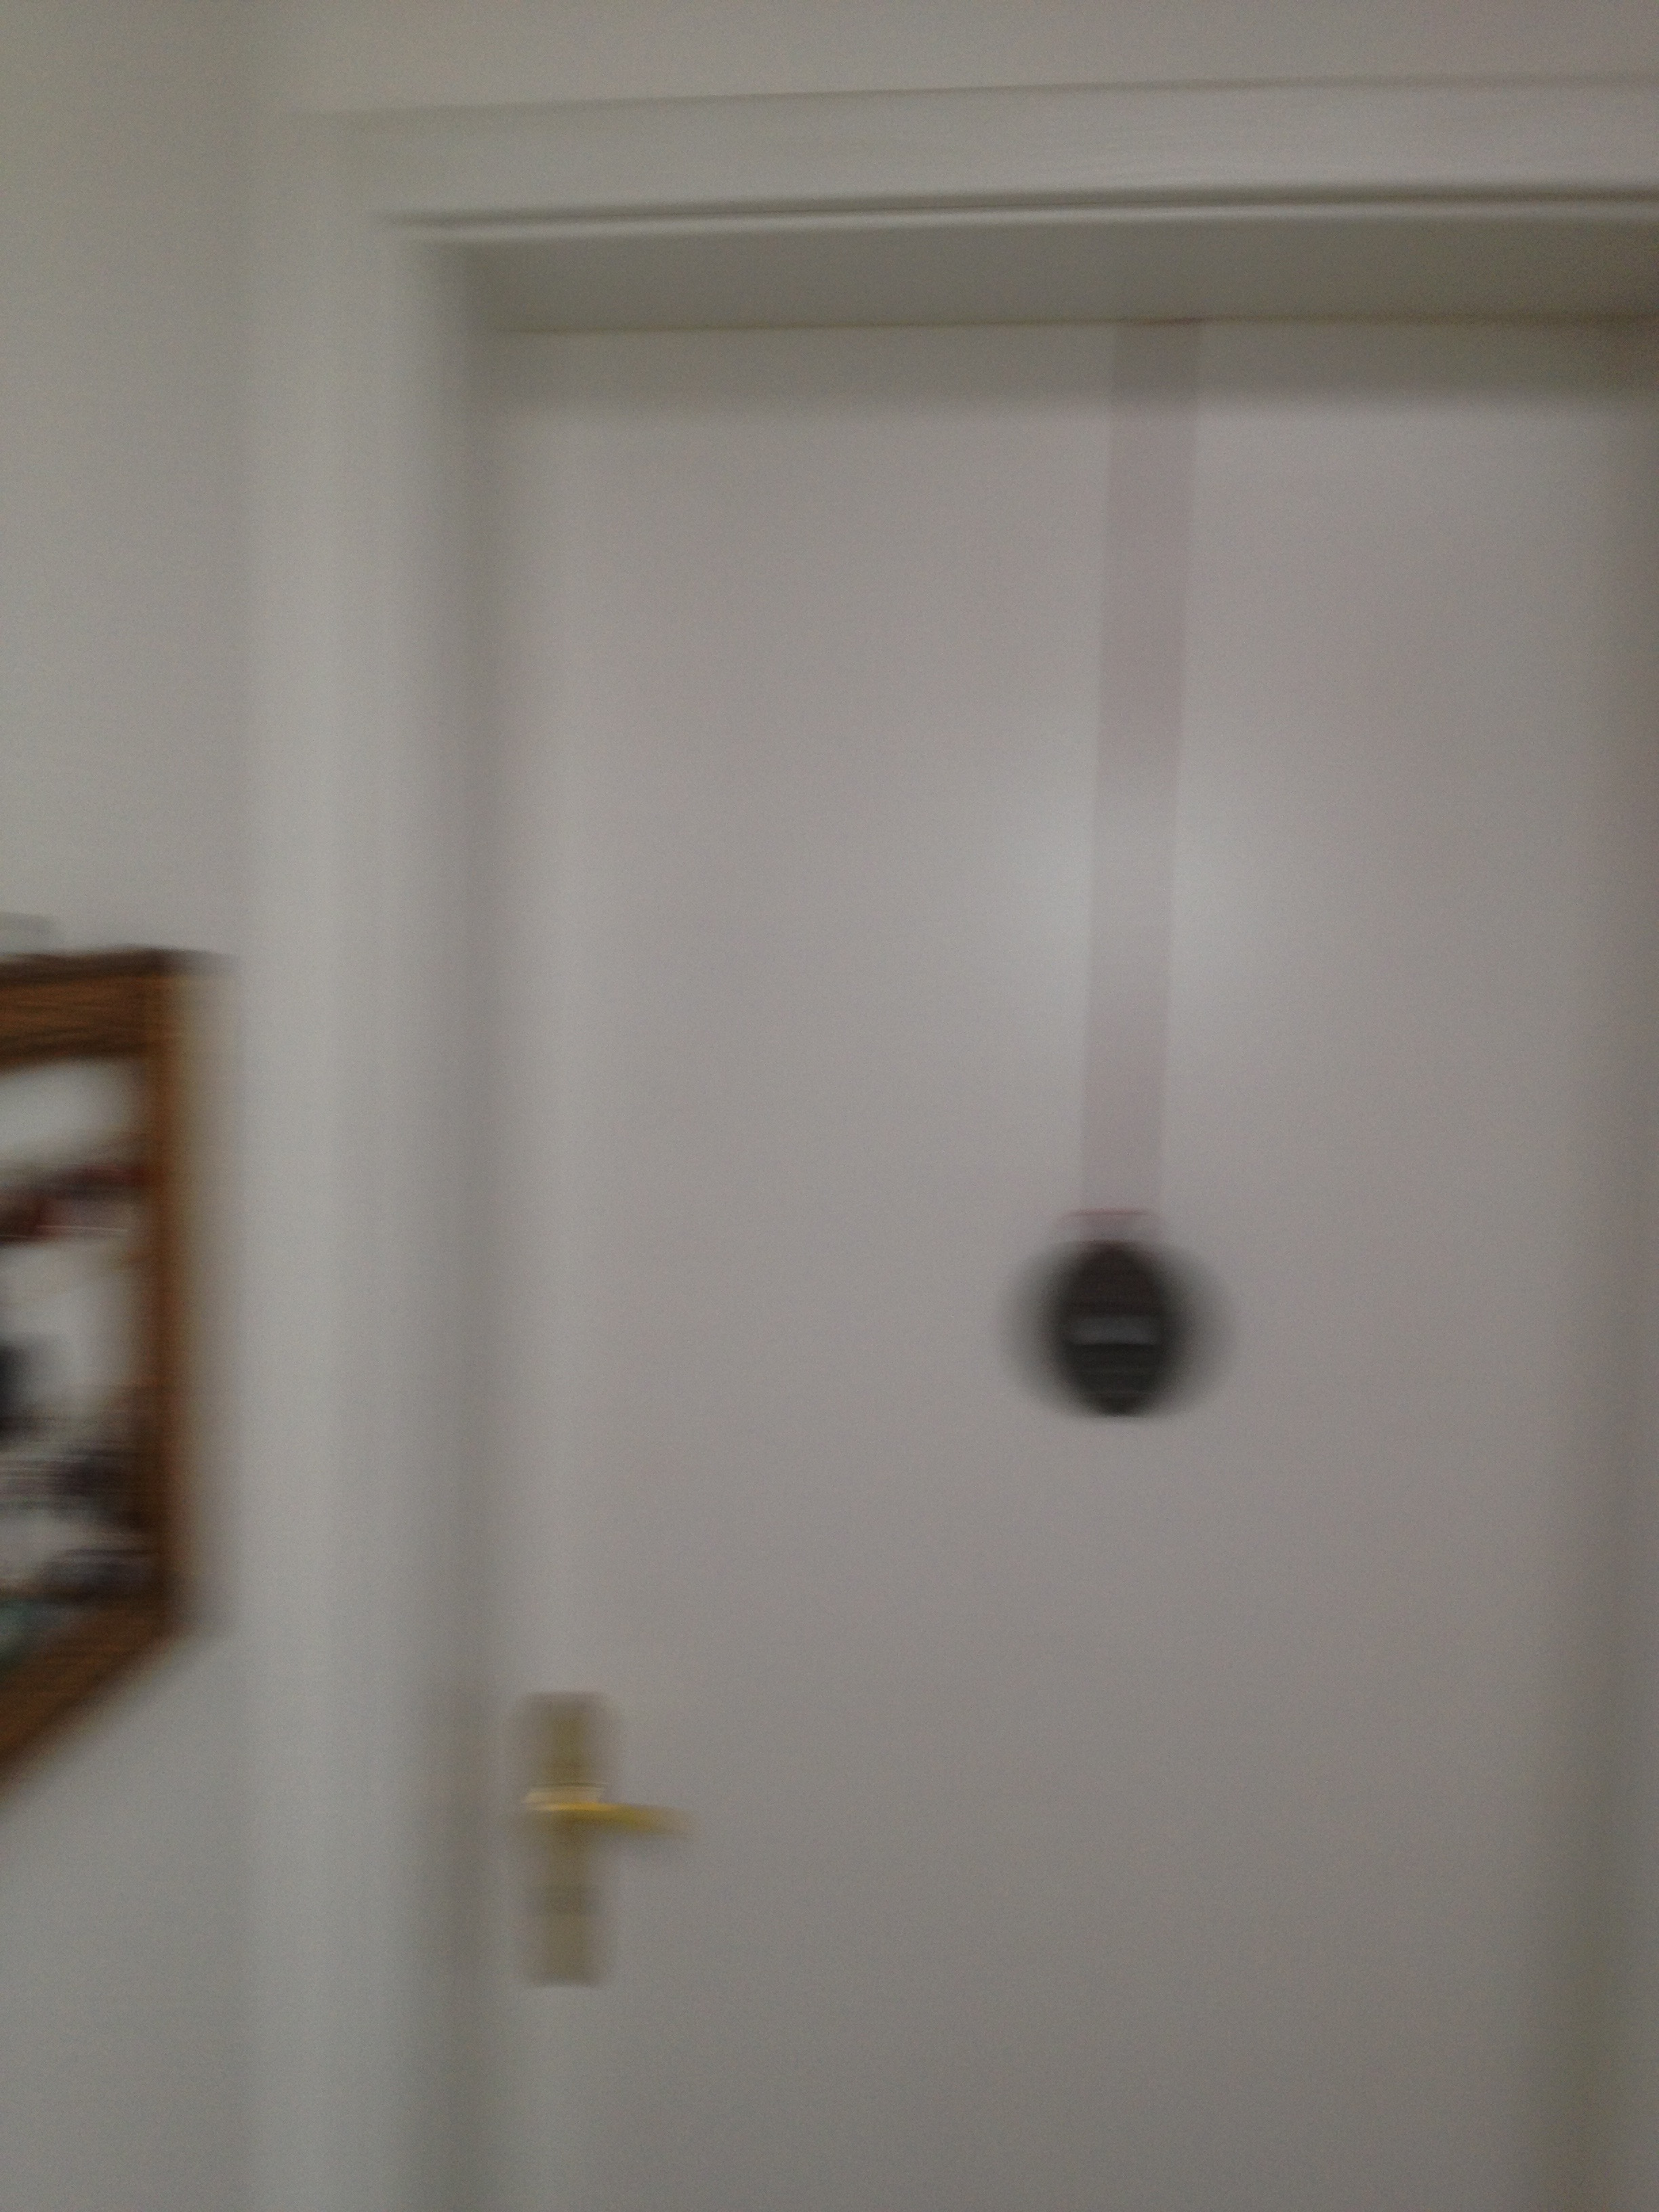
\includegraphics[width=7cm]{capture_1-5.jpg}
}
\end{center}
\caption{Translation entlang vermeintlicher y-Achse}
\label{fig:1-2}
\end{figure}

\begin{figure}[!htpb]
\begin{center}
\subfigure[Tageslicht]{
  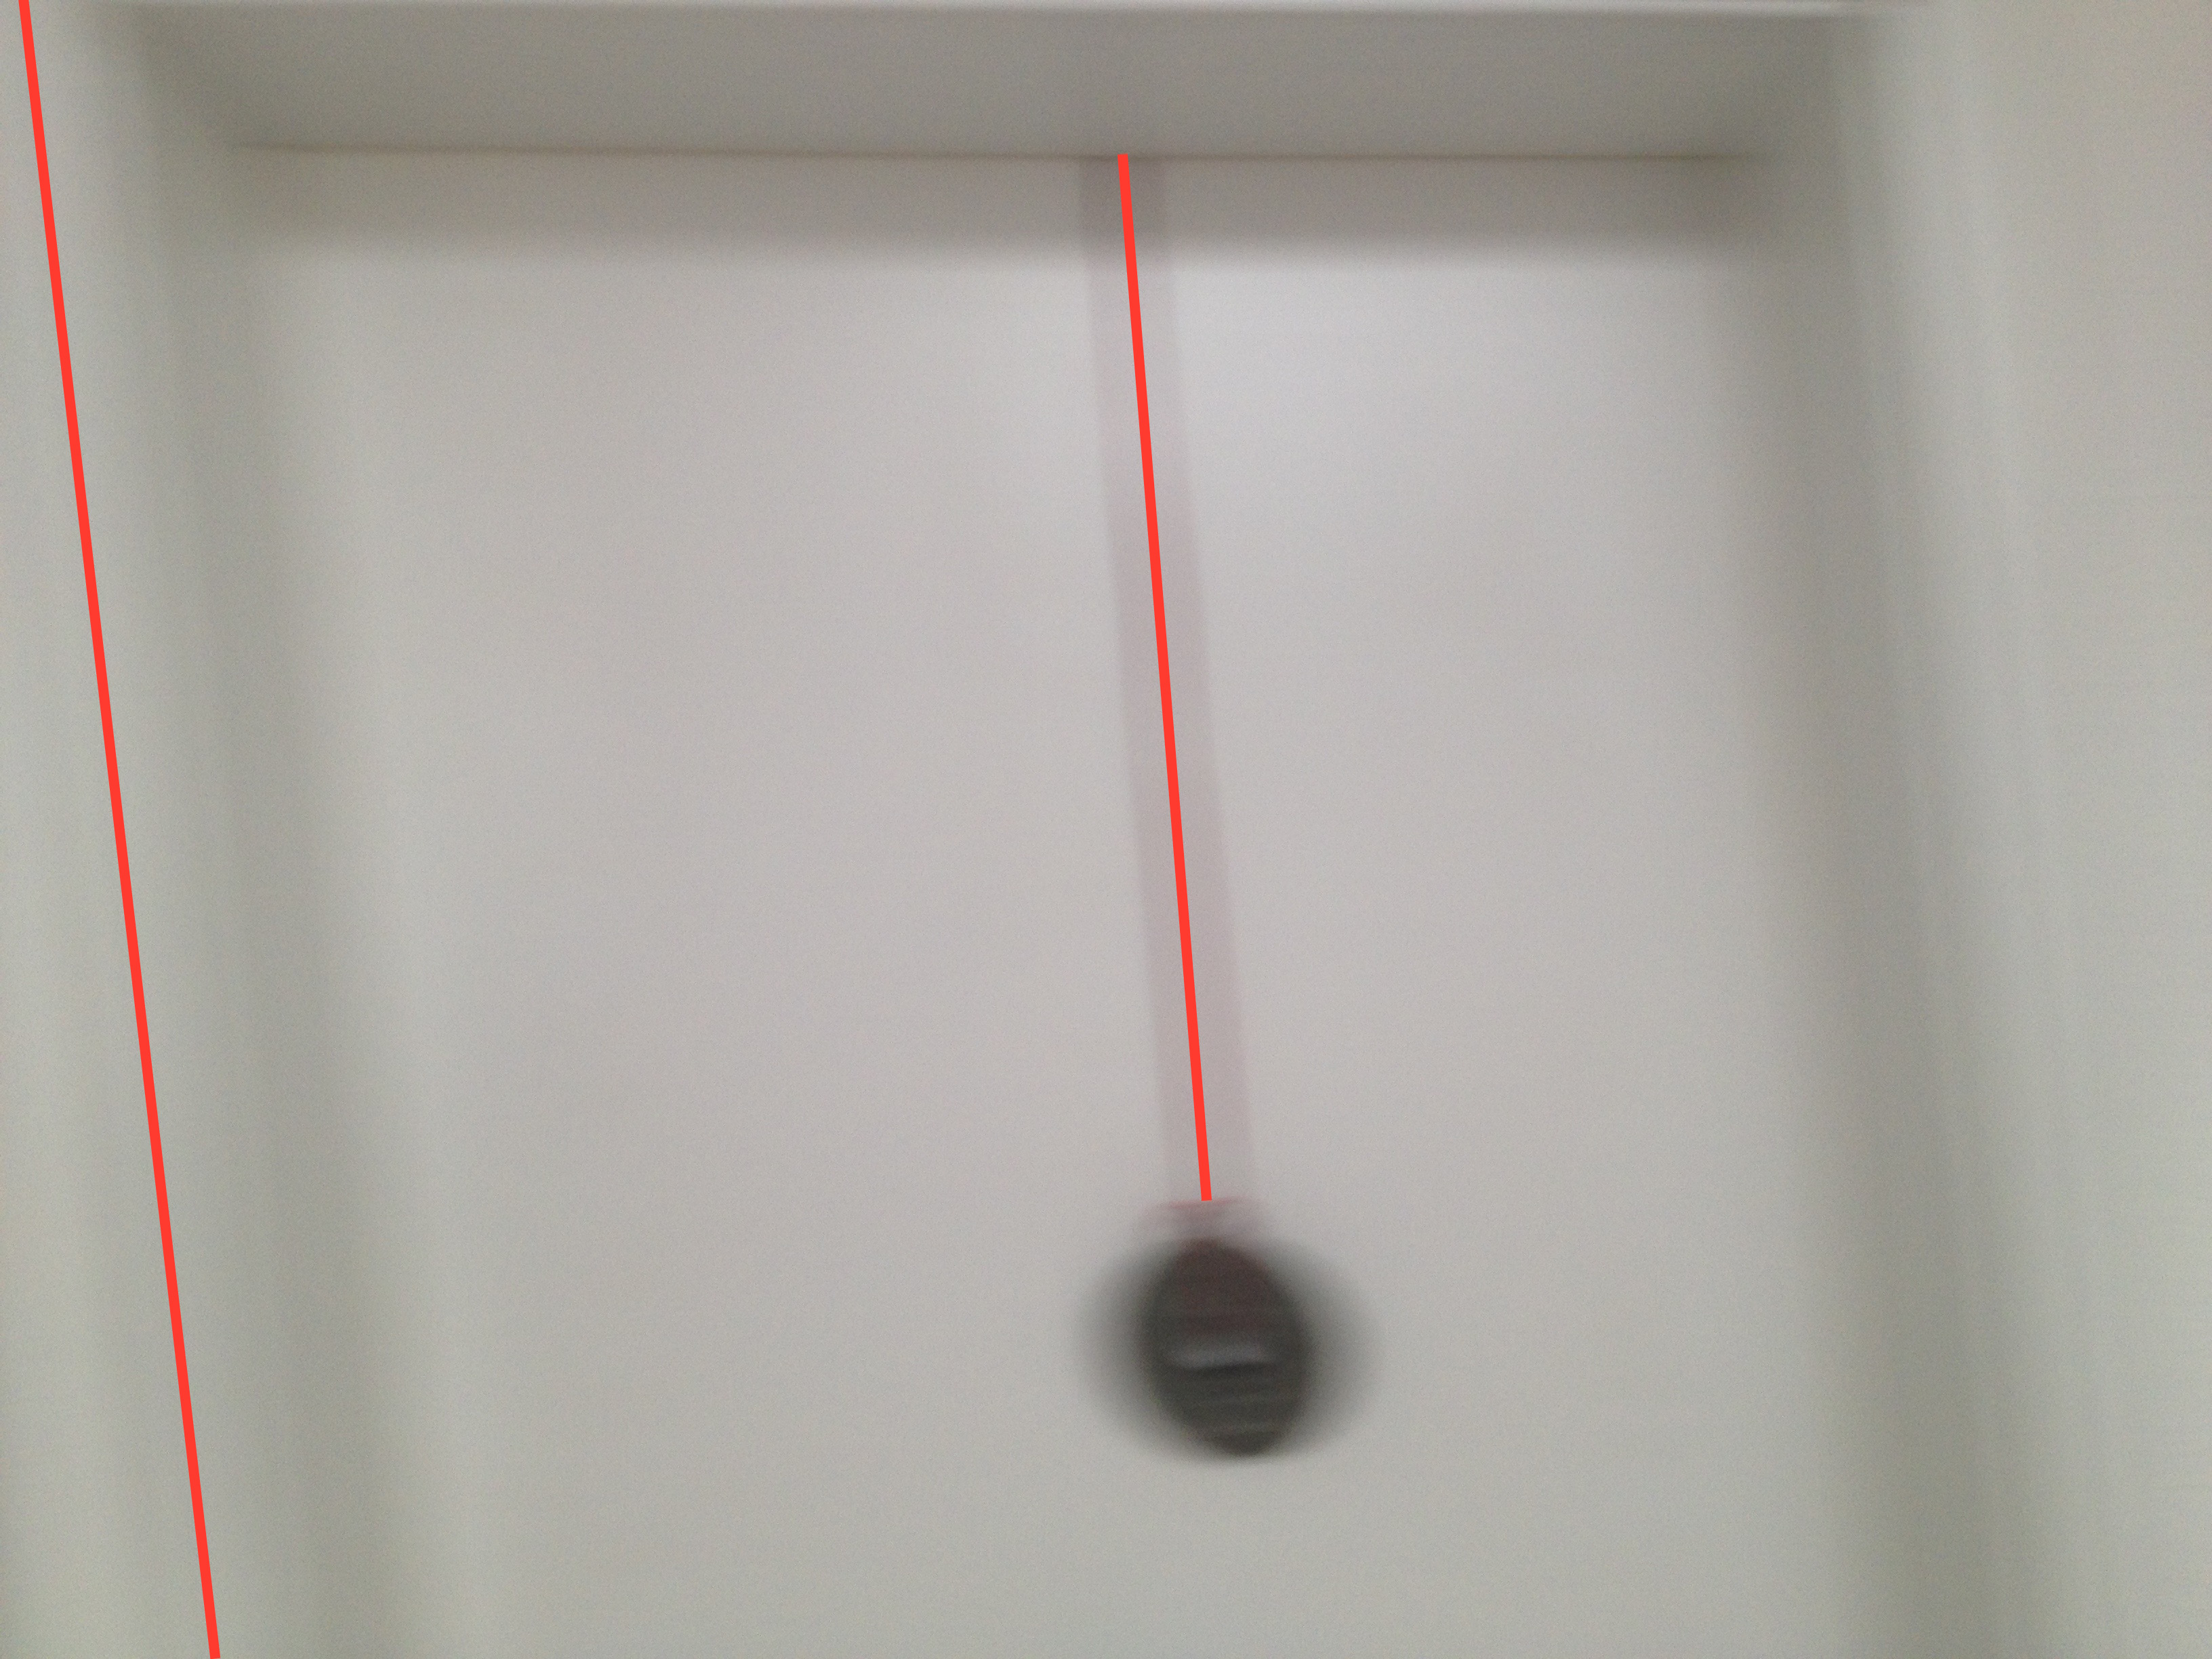
\includegraphics[width=7cm]{capture_1-3.jpg}
}
\subfigure[Blitz + Halogenspot]{
  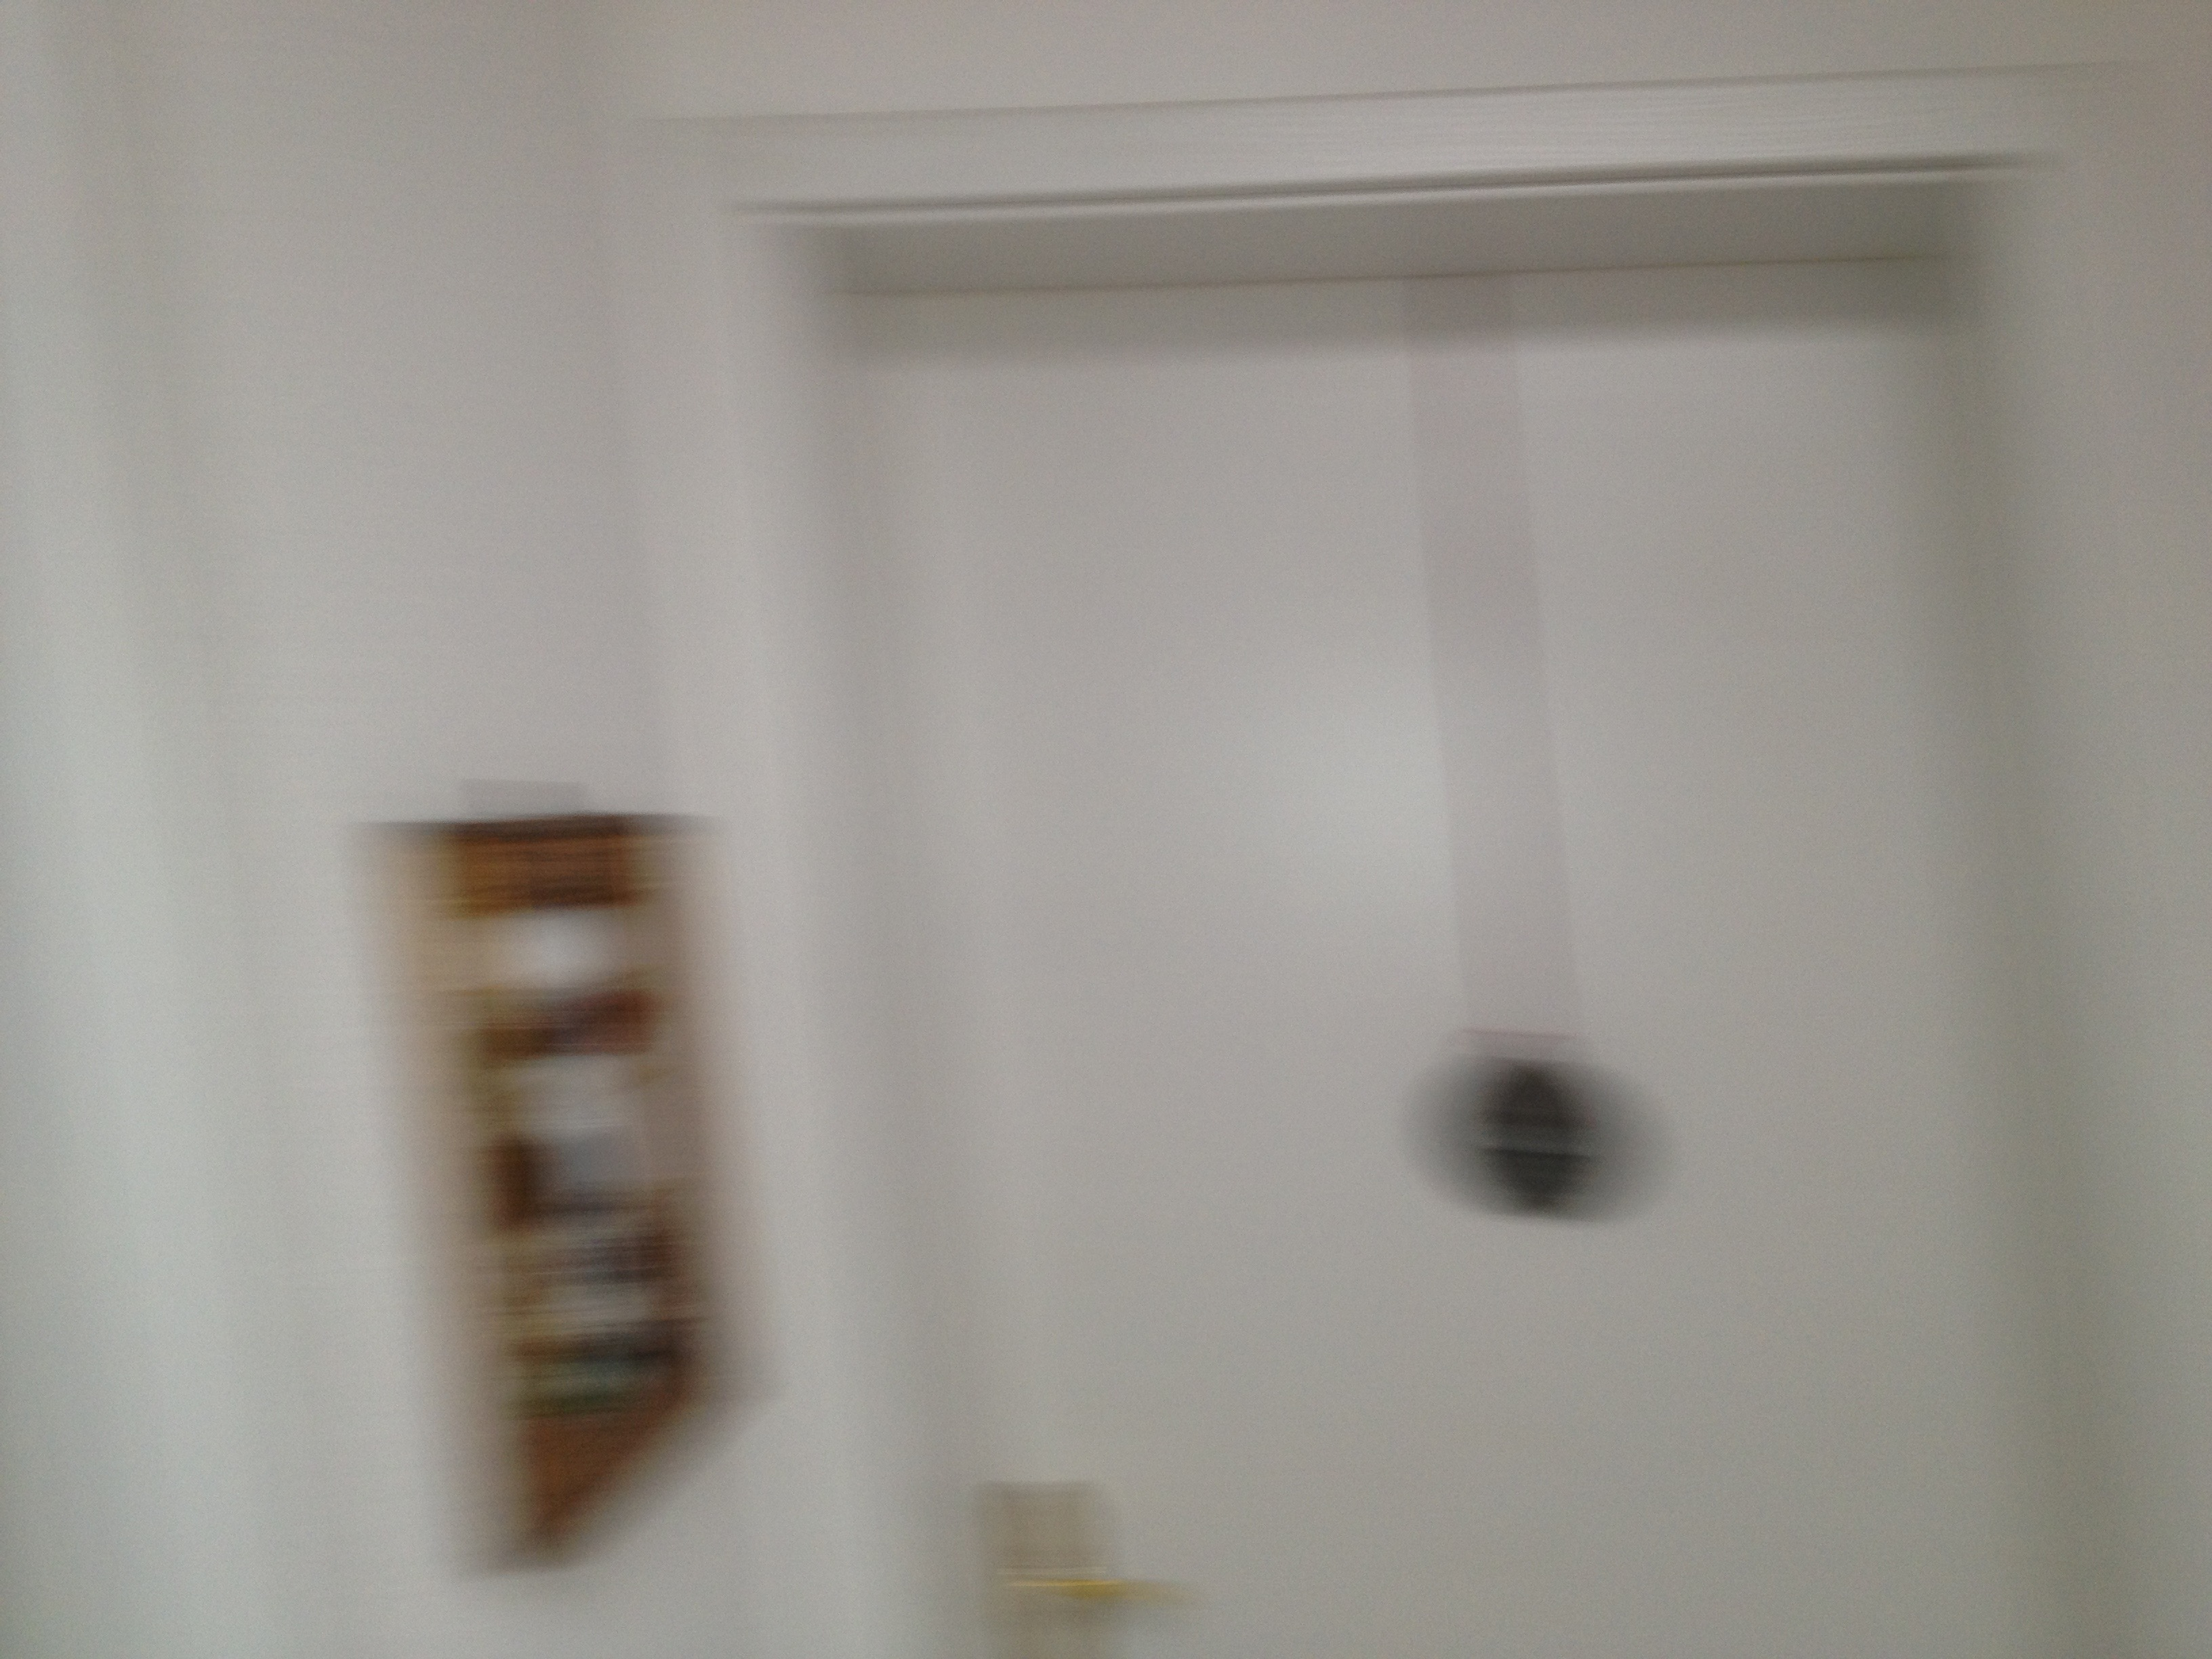
\includegraphics[width=7cm]{capture_1-6.jpg}
}
\end{center}
\caption{Translation entlang vermeintlicher x-Achse}
\label{fig:1-3}
\end{figure}

\begin{figure}[!htpb]
\begin{center}
\subfigure[Tageslicht]{
  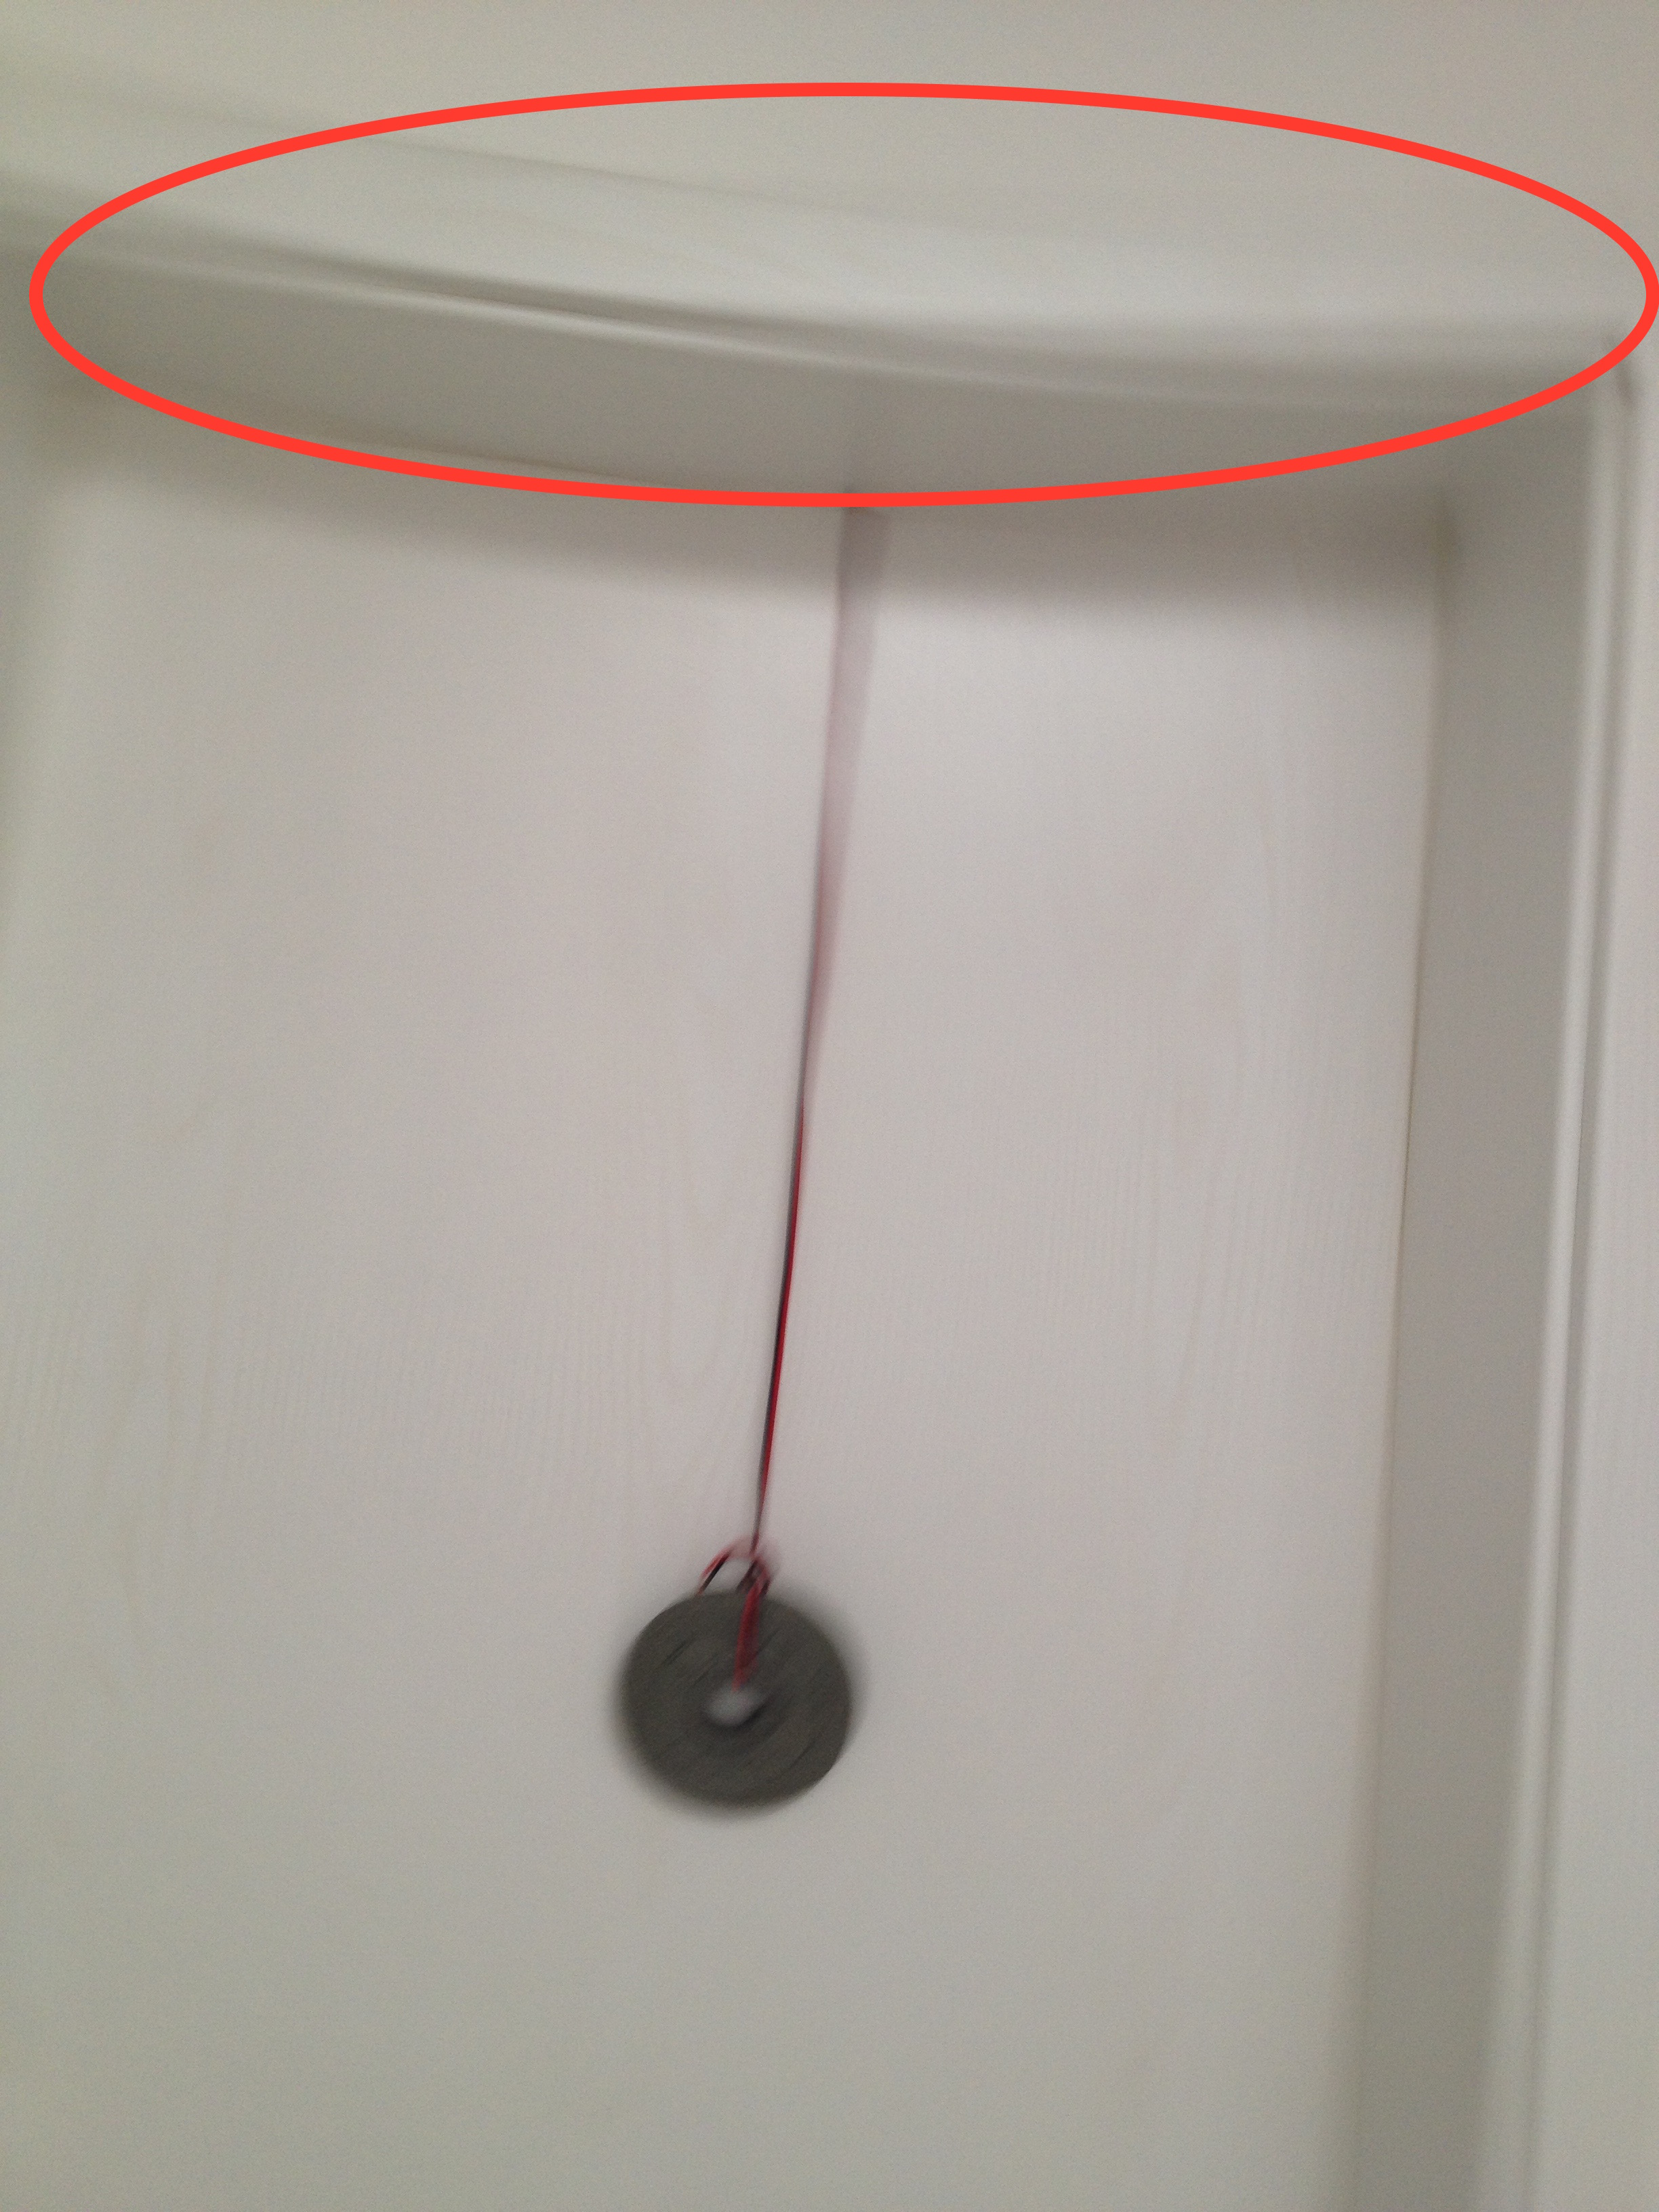
\includegraphics[width=7cm]{capture_1-4.jpg}
}
\subfigure[Blitz + Halogenspot]{
  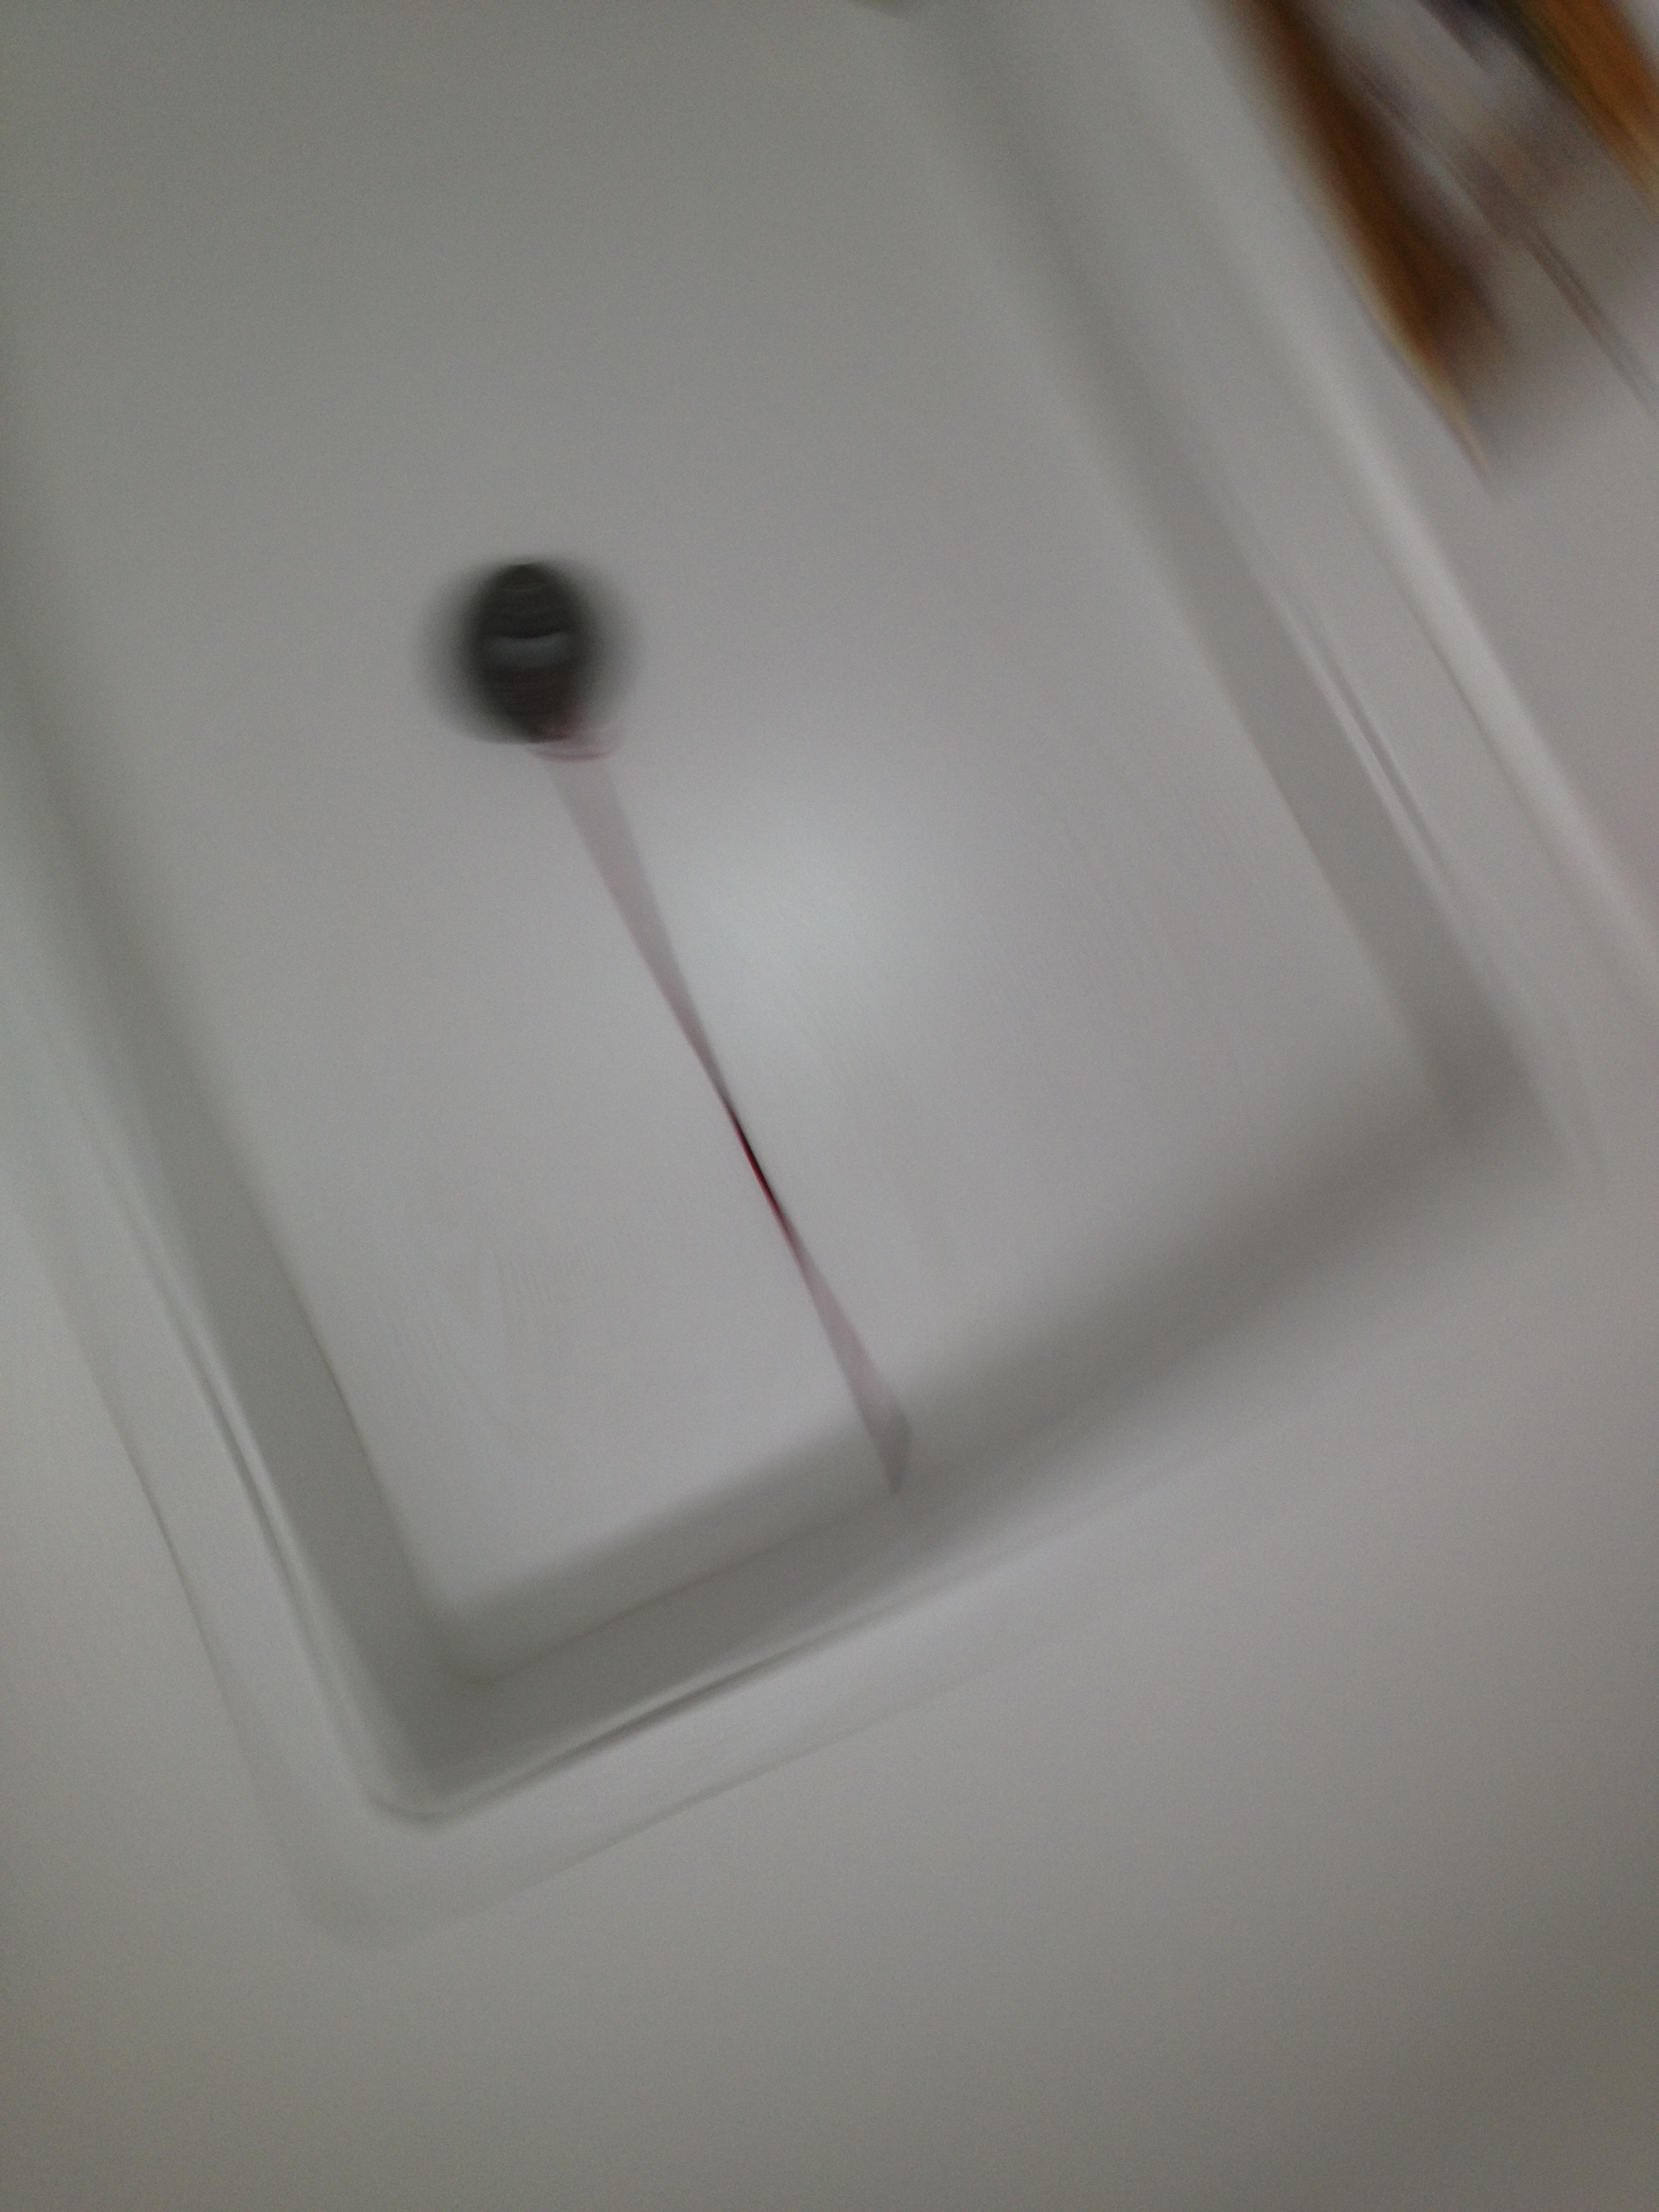
\includegraphics[width=7cm]{capture_1-7.jpg}
}
\end{center}
\caption{Rotation}
\label{fig:1-4}
\end{figure}
\end{task}

\newpage
\begin{task}{Pinhole-Kamera-Projektion}
\subtask{2.1}
\emph{Im Anhang zur Aufgabe findest Du eine Reihe von Weltpunkten im Kamerakoordinatensystem. Implementiere das Pinhole-Kameramodell und projiziere die Weltpunkte auf Deinen virtuellen Bildsensor.}

Da die Daten erfreulicherweise bereits in's Kamerakoordinatensystem transformiert wurden (Danke!) gehe ich davon aus, dass auch die Achsen derart gewählt wurden, dass kein zusätzliches Flippen oder Rotieren mehr erforderlich ist. Da nicht anders spezifiziert ist diese Annahme ja so gut wie jede andere.

Somit erfolgt die Projektion $p_c(x,y,z)$ eines Punktes $\begin{pmatrix}x\\y\\z\end{pmatrix}$ auf einen Punkt auf dem Bildsensor bei gegebener Brennweite $f$ straight-forward durch:
$$p_c(x,y,z)=\frac{f}{z}\cdot\begin{pmatrix}x\\y\end{pmatrix}$$
Abbildung \ref{fig:2-1} zeigt das Resultat für $f=5000$.

\begin{figure}[!htpb]
\begin{center}
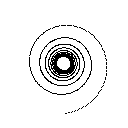
\includegraphics[width=9cm]{capture_2-1.png}
\end{center}
\caption{Projektion (Pinhole, $f=5000$)}
\label{fig:2-1}
\end{figure}

\subtask{2.2}
\emph{Verringere nun die Brennweite um die Hälfte. Projiziere erneut und überlagere die neue und alte Projektion.}

\begin{figure}[!htpb]
\begin{center}

\includegraphics[width=9cm]{capture_2-2.png}
\end{center}
\caption{Projektion (Pinhole, $f=2500$)}
\end{figure}

\begin{figure}[!htpb]
\begin{center}
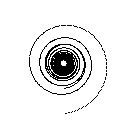
\includegraphics[width=9cm]{capture_2-3.png}
\end{center}
\caption{Die beiden Projektionen übereinander}
\end{figure}

\newpage
\subtask{2.3}
\emph{Verändere Deinen Code für die Parallelprojektion und nutze diese, um die Weltpunkte erneut auf den Sensor zu projizieren.}

Da keine Richtung für die Projektion spezifiziert ist, gehe ich davon aus, dass die Richtung der Projektion orthogonal zum Sensor ist. In diesem Fall ist die Projektion trivial (die $x,y$ - Koordinaten bleiben erhalten). Das Bild ist lediglich skaliert und auf die Abmessungen des pseudo-Sensors angepasst.

\begin{figure}[!htpb]
\begin{center}
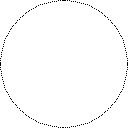
\includegraphics[width=7cm]{capture_2-4.png}
\end{center}
\caption{Projektion (parallel, Richtung orthogonal)}
\end{figure}
\end{task}

\newpage
\begin{task}{Bayer-2-Color}
\subtask{3.1}
\emph{Im Anhang zur Aufgabe findest Du eine Bildmatrix, die das rohe Bayer-Format aufweist. Die Breite des Bildes ist übrigens 1282 Pixel. Stelle ein Unterbild dar von (350, 180) bis (440, 260).}

\begin{figure}[!htpb]
\begin{center}
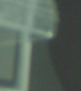
\includegraphics[width=7cm]{capture_3-2.png}
\end{center}
\caption{Teilbild in der Box zwischen $(350, 180)$ und $(440, 260)$}
\label{fig:3-2}
\end{figure}

\subtask{3.2}
\emph{Implementiere eine Funktion zur Erstellung eines Farbbildes aus den Rohdaten}

Ich habe linear interpoliert, also stets: die 9 Nachbarn eines Pixels betrachtet, gemäß des Mosaik-Musters $\begin{pmatrix}g&b\\r&g\end{pmatrix}$ die Farbe ermittelt, die dieser Nachbar repräsentiert und anteilig an der Anzahl der Nachbarn dieser Farbe den Wert lokal einfließen lassen.

Statt Einzelheiten gibt's aber auch hier ein Bild: Abbildung \ref{fig:3-1}.

\begin{figure}[!htpb]
\begin{center}
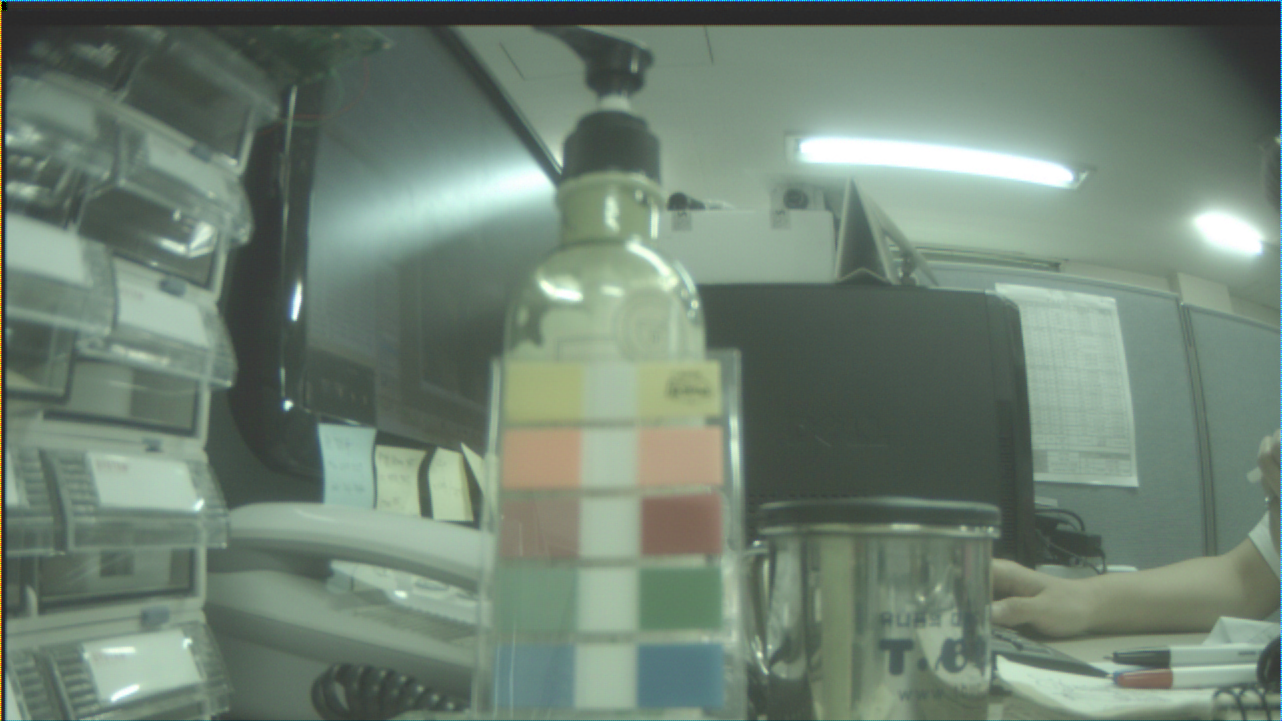
\includegraphics[width=14cm]{capture_3-1.png}
\end{center}
\caption{Bild in Farbe}
\label{fig:3-1}
\end{figure}

\emph{Welche Farbe hat der Stift rechts unten?}

Einer ist rot, der andere schwarz.
\end{task}
\end{document}